% !TeX encoding=utf8
% !TeX spellcheck=en-Us
\chapter{Setup}
This chapter presents the experimental setup for electroluminescence (EL) \hyphenation{mea-sur-ements}. Successful EL measurements consist of charge injection, charge recombination and luminescence detection. Therefore \autoref{sec:GeneralSetup} explaines the general setup. The following \autoref{sec:electricalconnection} explains the Perovskite Cell layout and electrical contacting of the cells. The emitted radiation is detected with a silicon ccd camera, which is explained with the additional optics in \autoref{sec:luminescencedetection}. The chapter concludes with the consideration of noise and errors.

\section{General Setup}\label{sec:GeneralSetup}
The setup is enclosed in black walls, shielding the inside from outside light and noise (see \autoref{fig:generalsetup}). All parts inside the chamber are painted black to minimizes noise and the detection of stray light. A vacuum pump, voltage source, multimeter and operating table with a computer are connected to the setup on the oustide, providing further utility. Inside the enclosre are the probe holder and camera (footnote - PCO sensicam). The Camera is can be moved in three dimension. Now we are going to look at the contact setup for PSCs.
\begin{figure}[h]
	\centering
	\includesvg{Images/ExperimentalSetup/ExperimentalSetupSketch.svg}
	\caption{Schematic of the EL measurement setup. Camera and Probe are positioned inside the setup and the computer, power supplies and measurement devices provided from the outside.}
	\label{fig:generalsetup}
\end{figure}


\section{Electrical Connection}\label{sec:electricalconnection}
Perovskite Solar Cells (PSCs) are manufactured on 25 mm x25 mm glass substrates (see \autoref{fig:perolayouttop}). Four cells are processed on one substrate, each single cell having dimensions of 4 mm x 3.5 mm. The cell stack consists of a glass substrate, with a xyz nm thick layer of Indium Tin Oxide (short ITO) deposited ontop. xyz nm of Spiro-TTB are used as a Hole Transport Layer (HTL), followed by 500 nm of Methylammonium-Lead-iodide (short MAPI) as the absorbing layer. The top side of the MAPI are contacted with xyz nm of C60 and BCP, acting as the Electron Transport Layer. In the end of the fabrication process, xyz nm Gold are deposited on top of the ITO and C60/BCP. Thus a holder with two pins, one on each gold pad, is needed to successfully contact the PSC. The used holder uses four pins, two to source voltage and two pins are used to check the contact.
\begin{figure}
	\centering
	\includesvg{Images/ExperimentalSetup/Pero_Layout_side}
	\caption{Schematic layout of the perovskite solar cell. Not to scale.}
	\label{fig:perolayouttop}
\end{figure}

The holder is electrically connected to a voltage supply (Kukusuki), in series with a 100 m$\Omega$ resistance, R, and two multimeters\footnote{Keithley 2000 Multimeter}. The multimeter measures the voltage drop across the resistor when current is sourced. The other multimeter measures the voltage drop U across the probe. The flowing current I is then calculated by Ohm's law:
\begin{equation}
	I = \frac{U}{R}
\end{equation}

Structured wells and a vacuum flange in the holder fixate the PSC on the holder. This ensures mechanical and electrical contact stability throughout the measurement.

This setup enables safe contacting of the probes inside the enclosure. After correct poling, charges are injected and recombine (radiatively). The emitted radiation has to be detected by a CCD Camera, what requires the usage of filters and optics.

\section{Luminescence detection}\label{sec:luminescencedetection}
In the setup filters and optics are used to select and focus the emitted radiation at a specific distance onto the imaging sensor. This chapter explains the used components and physical processes.
\subsection{Filters}
Between probe and sensor a filter\footnote{bk-Interferenzoptik, custom made product} is used to filter the wavelengths reaching the detector. Generally filters function by absorbtion or interference and can be used to either transmit or reflect specific wavelengths. The filter in the setup is a bandpass filter and thus only transmits wavelengths from 780-820 nm. This filter is sensitive to high intensity, ... , which is above/below the luminescence emission of the PSC. The bandpass wavelengths are chosen accordingly to the luminescence emission spectra from the perovskite (see \autoref{fig:spectrum_perofilter}). This enables maximum sensitivity to the emitted radiation and limits the detection of stray light.

\begin{figure}
	\centering
	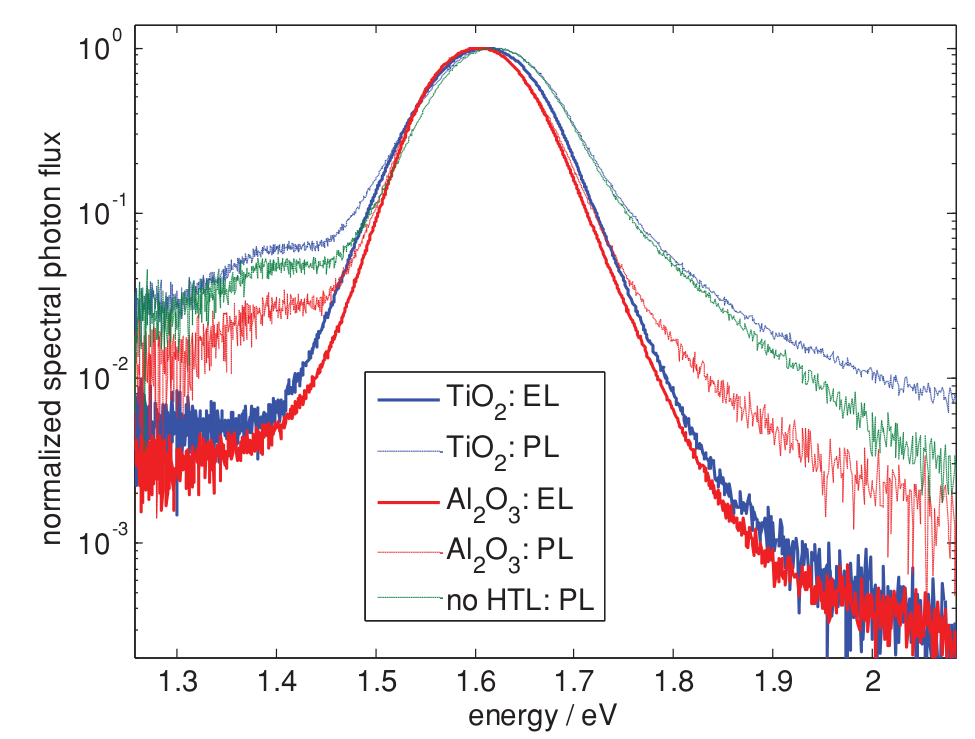
\includegraphics[width=0.7\linewidth]{Images/ExperimentalSetup/Perovskite_Spectrum}
	\caption{Emitted luminescence spectrum of the perovskite and transmission function of the filter. Taken from 2015 Predicting Voc.}
	\label{fig:spectrum_perofilter}
\end{figure}
\subsection{Optics}
Optics focus the radiation onto a charge coupled sensor (CCD). This setup uses a lens\footnote{Pentax, C2514-M (KP)} with a focus length of 14 mm and an aperature of 1.6. This focuses the 25x25 mm$^2$ to an approximate area of ..., with a pixel size of ... . A resolution of ... . 
\\
SKETCH FOR LENS SYSTEM
\\
Special optics are used to limit erros as abberation,... ,?

\subsection{Charge Coupled Detectors}
The radiation is focused onto a CCD sensor\footnote{Sony ICX285-AL} in a camera\footnote{PCO, sensicam qe}. CCD Sensors are silicon chips structured into small squares, called wells (see \autoref{fig:ccdsensor}). The number of wells correspond to the number of pixel in the taken picture. Radiation generates charges, electrons and holes, and externally applied voltages seperate and trap the charges in the wells. For a specific time, called exposure time, radiation hits the sensor and charges accumulate in the wells. The amount of generated electrons per incoming photon is called the quantum efficiency, and depends on the sensor material and energy of the photon. After the exposure time a series of voltages is applied to shift the charges from the light sensitive wells to opaque covered wells. Then the charges are extracted row by row and the voltage of each well is measured. An A/D converter convertes the voltage into an Digital signal, which is saved and later processed.
\begin{figure}
	\centering
	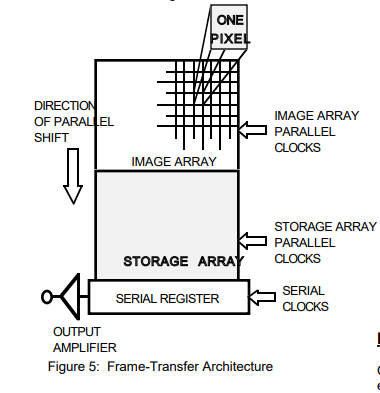
\includegraphics[width=0.7\linewidth]{Images/ExperimentalSetup/CCD_Sensor}
	\caption{Schematic represantation of a CCD sensor. Taken from kodak primer.}
	\label{fig:ccdsensor}
\end{figure}

This process spacially measures the radiation intensity. However several sources of errors occur, which are checked further.
The quantum efficiency for the used camera peaks at 500 nm and decays for larger wavelengths (compare \autoref{fig:pcosensicamqe}). This reduces the sensitivity for EL detection in the range of around 800 nm to about 10 \%, however still suffices.
\begin{figure}
	\centering
	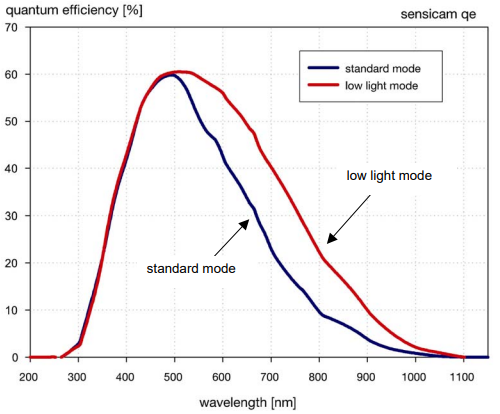
\includegraphics[width=\linewidth]{Images/ExperimentalSetup/PCO_sensicam_QE}
	\caption{Quantum efficiency of the PCO sensicam qe, given by the manufacturer.}
	\label{fig:pcosensicamqe}
\end{figure}

\section{Noise and measurement errors}
Several sources of errors can deviate the measured signal from physical value. In the readout process of the CCD sensor, these correspond to dark noise, readout noise and hot or cold pixel. Dark noise corresponds to the thermal generation of electrons. To reduce this the CCD sensor is cooled to -12°C. The measurement of dark images, images without illumination or applied voltage, and subtracting them from the EL image, allow further reduction of dark noise. Because of this, the EL images shown in this work are already corrected by dark noise.\\

Other sources of errors happen when shifting the electrons from well to well, called readout noise. This are given by the manufacturer and need to be taken into account.
 